% ----- INPUT
% same as raster
\newcommand{\fcrasterimageh}{0.2632887\textwidth}
% 2.8165 * height
\newcommand{\fcrasterimagew}{0.74155\textwidth}

% to shift for ticks
\newcommand{\fcrastershiftx}{1.3em}
\newcommand{\fcrastershifty}{1em}

% to shift to the middle from kinda the middle
\newcommand{\fcrastermidshiftx}{0.5em}
\newcommand{\fcrastermidshifty}{0.4em}

%
\newcommand{\fcrasterhormid}{0.5 * \fcrasterimagew}
\newcommand{\fcrastervermid}{0.5 * \fcrasterimageh}



\begin{tikzpicture}[
        arr/.style = { -{Stealth[ ]} },
        bluearrow/.style = {arr, draw=third-color, fill=third-color, thick},
        blackarrow/.style = {arr, ultra thick},
    ]
    
    \begin{scope}

        \node[
            shift={(\fcrastermidshiftx, -\fcrastershifty)}
        ] at (\fcrasterhormid, 0) {{ \small Time}};
        
        \node[
            shift={(-\fcrastershiftx, \fcrastermidshifty)},
            rotate=90
        ] at (0, \fcrastervermid) {{\small Frequency}};

        
        % \node[shift={(\apwest, \apshifth)}, anchor=west] at (0, \appeakh) {peak};
        
    \end{scope}
    
    \begin{scope}
        \node[anchor=south west,inner sep=0] at (0,0) {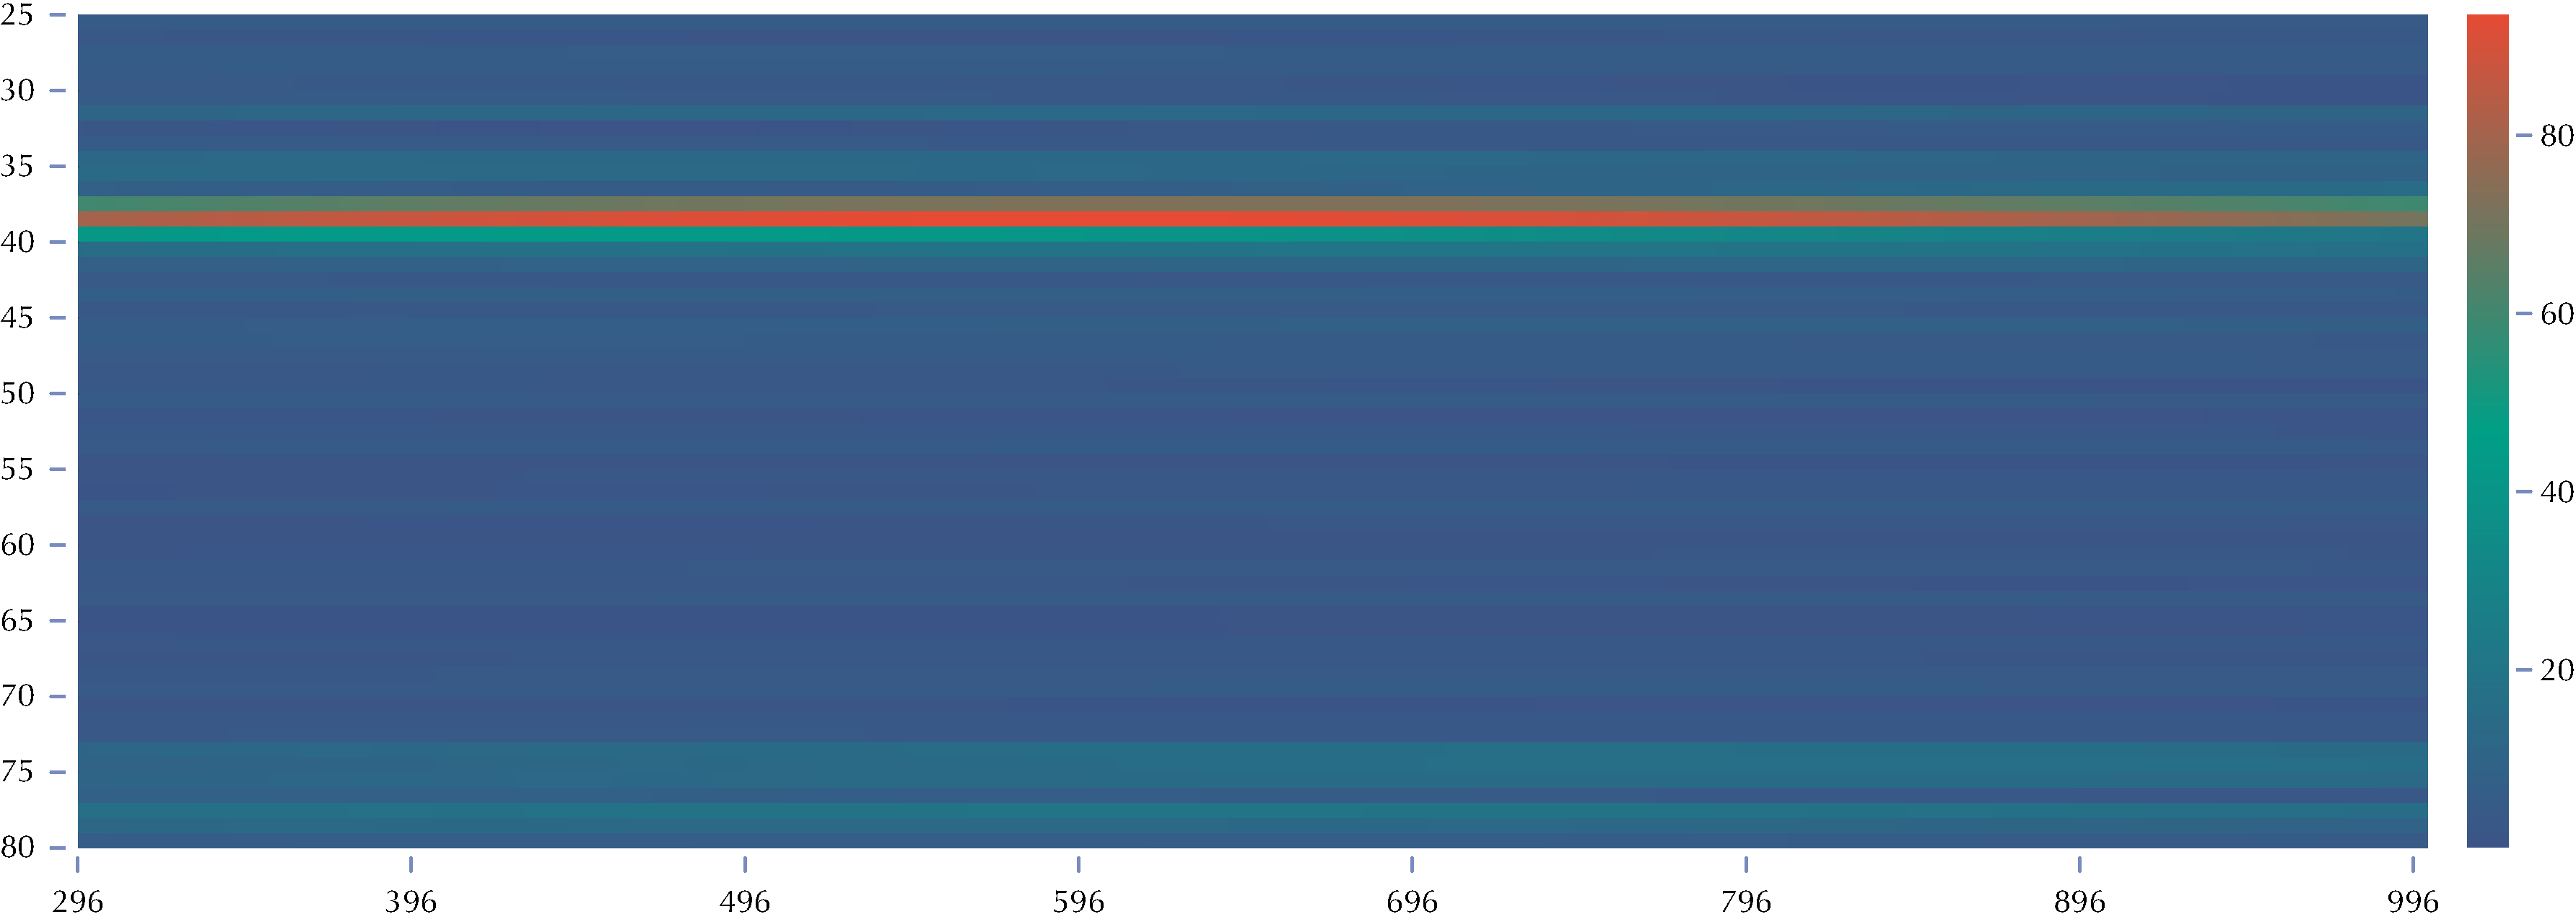
\includegraphics[height=\fcrasterimageh]{src/assets/images/14/tfr14.pdf}};
    \end{scope}
        
\end{tikzpicture}